\section{什么是目标检测}

\begin{frame}[allowframebreaks]
    \frametitle{\textsc{目录}} \vspace{-0.3cm}
    \begin{spacing}{0.0}
        \tableofcontents[currentsection,hideallsubsections]
    \end{spacing}   % 若不想要目录, 注释掉该句
\end{frame}



\begin{frame}
    \noindent\large\textbf{目标检测}
    \vspace{0.4cm}
    \begin{itemize}
        \item[$ \bullet $] 是什么?
        \item[$ \bullet $] 在哪里?
        \item[$ \bullet $] 有哪些?
    \end{itemize}
    \vspace{1cm}
    “是什么”意味着需要判断出找出来的目标是什么,也就是对目标的类别做判断,是人还是狗或者是车\\
    \vspace{1em}
    “在哪里”需要指出找到的目标在图像的那个地方,范围是哪里\\
    \vspace{1em}
    “有哪些”意味着需要将图像当中所有的感兴趣物体(预先定义的类别)找出来\\
\end{frame}

\begin{frame}
    \noindent\large\textbf{如何表示}\\
    在计算机当中需要用数字来表达“是什么”、“在哪里”、“在哪里”
    \vspace{1em}
    \begin{itemize}
        \item[$ \bullet $] 整数(one-hot 向量)表示类别
        \item[$ \bullet $] 矩形框表示位置(四元组$[x,y,w,h]$)
        \item[$ \bullet $] 堆叠所有目标组成数组$n\times5$
    \end{itemize}
    \vspace{1em}
    \begin{figure}
        \subfloat[box]{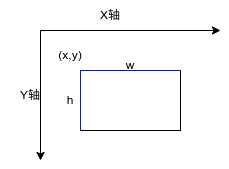
\includegraphics[width=0.4\linewidth]{box.png}}
        \hspace{1cm}
        \subfloat[Object Detection]{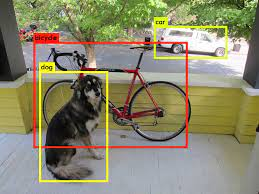
\includegraphics[width=0.4\linewidth]{obd1.jpg}}
    \end{figure}
\end{frame}

\begin{frame}
    \noindent\large\textbf{基础知识}
    \begin{itemize}
        \item[$ \bullet $] 矩形框的3种表示
            矩形框的表示形式有:\\
            $[x,y,w,h]$ \\
            $[x_1,y_1,x_2,y_2]([left,top,right,bottom])$\\
            $[cx,cy,w,h]$
        \item[$ \bullet $] 交并比(IoU)
            交并比是指两个矩形的交集与并集的面积之比$IoU=\frac{|A\cap B|}{|A\cup B|}$,
            实现是采用第二种矩形表示进行实现$A[l_A,t_A,r_A,b_A],B[l_B,t_B,r_B,b_B]$:\\
            $S_A=(r_A-l_A)\times(b_A-t_A)$\\
            $S_B=(r_B-l_B)\times(b_B-t_B)$\\
            $W_{AB}=(min(r_A,r_B)-max(l_A,l_B))$\\
            $H_{AB}=(min(b_A,b_B)-max(t_A,t_B))$\\
            if $ W_{AB}<0$ or $H_{AB}<0$ then $IoU = 0$\\
            else $IoU=\frac{W_{AB}\times H_{AB}}{S_A+S_B-W_{AB}\times H_{AB}}$
            % \hspace{10cm}
            \vspace{-3.5cm}
            \begin{figure}
                \hspace{6cm}
                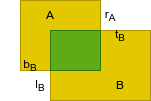
\includegraphics[width=0.4\linewidth]{iou.png}
            \end{figure}

    \end{itemize}
\end{frame}


\begin{frame}
    \noindent\large\textbf{常见数据集}

    %    \begin{itemize}
    %    \item[$ \bullet $]  包含图像和标签(掩码、mask、Ground Truth)
    %
    %    %\vspace{1em}
    %    \item[$ \bullet $]  图像与标签大小相同
    %
    %    %\vspace{1em}
    %    \item[$ \bullet $]  图像与标签的像素一一对应
    %
    %    %\vspace{1em}
    %    \item[$ \bullet $] 标签的形式多种多样,包括图像、描述文件、表格等形式
    %    \end{itemize}
    %
    %    \vspace{1em}
    %    \noindent\large\textbf{常见数据集}

    \vspace{1em} \small
    Common Objects in COntext(COCO)、PASCAL Visual Object Classes(PASAL)
\end{frame}



\begin{frame}
    \noindent\large\textbf{常用评价指标}

    \vspace{0.1em}
    $\bullet$ 准确率:$PA=\frac{TP+TN}{TP+FP+FN+TN}$

    \vspace{0.1em}
    $\bullet$ Dice系数(Dice score, F1分数):$dice(A,B)=\frac{2|A\cap B|}{|A|+|B|}=\frac{2TP}{2TP+FN+FP}$

    \vspace{0.1em}
    $\bullet$ 雅卡尔指数(交并比):$IoU=\frac{|A\cap B|}{|A \cup B|} = \frac{TP}{TP + FN + FP}$

    \vspace{0.1em}
    $IoU= \frac{Dice}{2-Dice}$; A: 目标像素的集合;B: 算法判定为目标像素的集合。除此之外还有精确率、召回率、平均准确率、平均精确率、平均召回率和聚合雅卡尔指数等指标

    \begin{figure}
        \subfloat[TP、FP、FN]{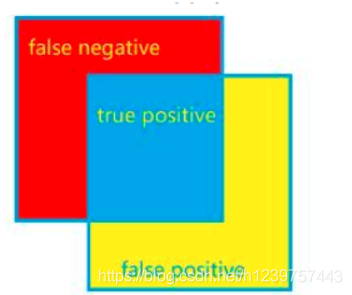
\includegraphics[width=0.3\linewidth]{TPFPFN.png}}
        \subfloat[IoU与Dice]{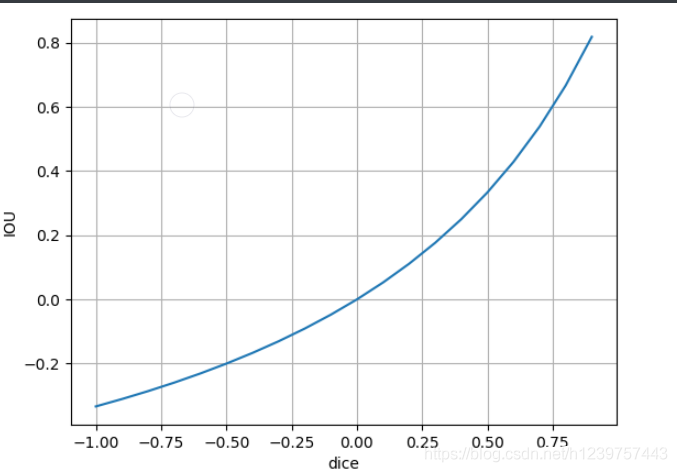
\includegraphics[width=0.3\linewidth]{IoUDice.png}}
    \end{figure}

\end{frame}

\begin{frame}
    \noindent\large\textbf{类别不平衡问题}

    \vspace{1em}
    图像当中的背景与前景常存在像素点数量不平衡的问题,这容易导致模型将所有像素点预测为同一个类别
    \begin{figure}
        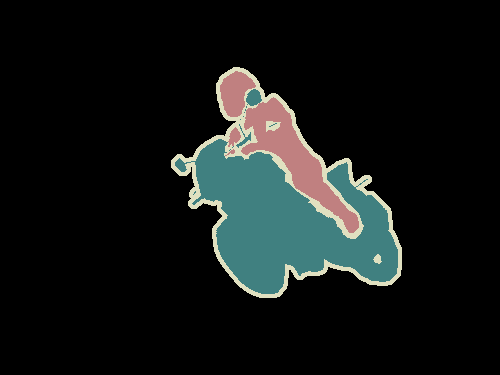
\includegraphics[width=8.0cm]{11.png}
    \end{figure}
\end{frame}

\begin{frame}
    \noindent\large\textbf{解决方法}

    \vspace{1em}
    $\bullet$ 损失函数加权:$L=\sum w_iloss_i$

    \vspace{1em}
    $\bullet$ 欠采样:样本多的类别只统计一部分像素点的损失

    \vspace{1em}
    $\bullet$ Dice损失函数:$L=1-\frac{2\sum \hat{y}_iy_i+\epsilon}{\sum (\hat{y}_i+y_i)+\epsilon}$

    \vspace{1em}
    $\bullet$ Focal损失函数:$L=-\sum (1-\hat{y}_i)^\gamma log(\hat{y}_i)$


\end{frame}

\begin{frame}
    \noindent\large\textbf{图像分割的应用}

    \vspace{1em}
    $\bullet$ 自动驾驶:对周围环境图像进行分割

    \vspace{1em}
    $\bullet$ 医学图像病灶检测:将医学影像当中的病变部位分割出来

    \vspace{1em}
    $\bullet$ 零售图像识别:对货架商品进行监控

    \vspace{1em}
    $\bullet$ 人脸识别:从图像当中提取人脸区域
\end{frame}

